% \documentclass[UTF8,12pt]{article} % 12pt 为字号大小
\documentclass[12pt]{article}
\usepackage[utf8]{inputenc}
\usepackage{amssymb,amsfonts,amsmath,amsthm}
\usepackage{cite}
%\usepackage{fontspec,xltxtra,xunicode}
%\usepackage{times}

%----------
% 定义中文环境
%----------

\usepackage{xeCJK}

\setCJKmainfont[BoldFont={Heiti SC Light},ItalicFont={Kaiti SC Regular}]{Songti SC Regular}
\setCJKsansfont{Heiti SC Light}
\setCJKfamilyfont{song}{Songti SC Regular}
\setCJKfamilyfont{zhhei}{Heiti SC Light}
\setCJKfamilyfont{zhkai}{Kaiti SC Regular}
\setCJKfamilyfont{zhfs}{STFangsong}
\setCJKfamilyfont{zhli}{Libian SC Regular}
\setCJKfamilyfont{zhyou}{Yuanti SC Regular}

\newcommand*{\songti}{\CJKfamily{zhsong}} % 宋体
\newcommand*{\heiti}{\CJKfamily{zhhei}}   % 黑体
\newcommand*{\kaiti}{\CJKfamily{zhkai}}  % 楷体
\newcommand*{\fangsong}{\CJKfamily{zhfs}} % 仿宋
\newcommand*{\lishu}{\CJKfamily{zhli}}    % 隶书
\newcommand*{\yuanti}{\CJKfamily{zhyou}} % 圆体

%----------
% 版面设置
%----------
%首段缩进
\usepackage{indentfirst}
\setlength{\parindent}{2em}

%行距
\renewcommand{\baselinestretch}{1.4} % 1.4倍行距

%页边距
\usepackage[a4paper]{geometry}
\geometry{verbose,
  tmargin=2cm,% 上边距
  bmargin=2cm,% 下边距
  lmargin=3cm,% 左边距
  rmargin=3cm % 右边距
}


%----------
% 其他宏包
%----------
%图形相关
\usepackage[x11names]{xcolor} % must before tikz, x11names defines RoyalBlue3
\usepackage{graphicx}
\usepackage{pstricks,pst-plot,pst-eps}
\usepackage{subfig}
\def\pgfsysdriver{pgfsys-dvipdfmx.def} % put before tikz
\usepackage{tikz}
\usepackage{float}

%链接相关
\usepackage[colorlinks,linkcolor=black,anchorcolor=blue,citecolor=green]{hyperref}

%原文照排
\usepackage{verbatim}

%网址
\usepackage{url}

%算法相关
\usepackage{algorithm}
\usepackage{algorithmicx}
\usepackage{algpseudocode}

\floatname{algorithm}{算法}
\renewcommand{\algorithmicrequire}{\textbf{输入:}}
\renewcommand{\algorithmicensure}{\textbf{输出:}}

%----------
% 习题与解答环境
%----------
%习题环境
\theoremstyle{definition} 
\newtheorem{exs}{习题}

%解答环境
\ifx\proof\undefined\
\newenvironment{proof}[1][\protect\proofname]{\par
\normalfont\topsep6\p@\@plus6\p@\relax
\trivlist
\itemindent\parindent
\item[\hskip\labelsep
\scshape
#1]\ignorespaces
}{%
\endtrivlist\@endpefalse
}
\fi

\renewcommand{\proofname}{\it{证明}}


%==========
% 正文部分
%==========

\begin{document}

\title{平时作业2}
\author{1160300314 朱明彦}
\date{\today} % 若不需要自动插入日期,则去掉前面的注释;{ } 中也可以自定义日期格式
\maketitle

\section{作业要求}
基于统计的异常探测问题中,有一种非参数方法称为直方图异常检测法。
如图\ref{fig:demand}所示,通过按照数据范围进行划分,将数据分配到相应的直方图中,可以统计出每个直方图中数据所占的比例。

\begin{figure}[H]
  \centering
  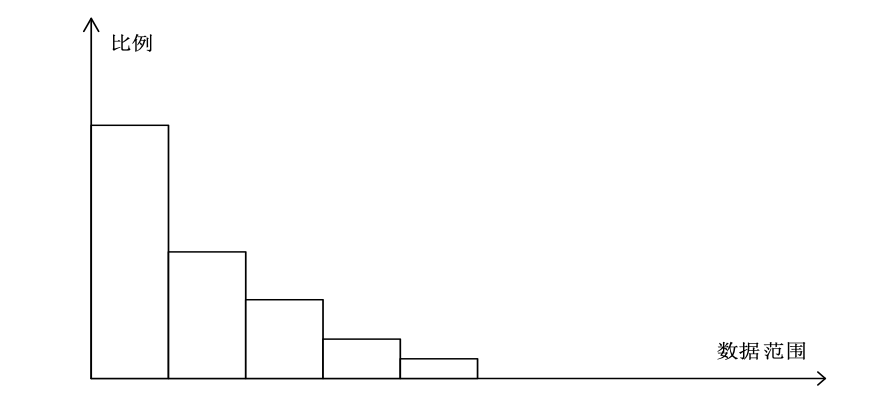
\includegraphics[width=0.8\linewidth]{fig/demand.png}
  \caption{直方图示意}
  \label{fig:demand}
\end{figure}

请设计一种算法,利用直方图进行异常检测
\begin{itemize}
  \item 给出构造直方图和检测异常点的主要步骤。
  \item 给出异常得分的计算公式。
\end{itemize}

\section{作业解答}
\subsection{主要步骤}
以下算法伪代码参考\cite{goldstein2012histogram}给出。

\begin{algorithm}[H]
  \caption{基于直方图的异常检测算法}
  \begin{algorithmic}[1]
    \Require 原始数据集合$S$, $N$为$S$的大小, $d$为每个原始数据的维度, $k$每个维度桶数
    \Ensure HBOS(Histogram-based Outlier Score)
    \Function {HBOS\_cal}{$S$, $N$, $d$, $k$, 样本$p$}
    \State $result \gets 0, i \gets 0$
    \While{$i < d$}
    \State $histogram_i$ = \Call{GetHistogram}{$S$, $N$, $i$, $k$}
    \State $result = result + \log\left(\frac{1}{histogram_{i}(p)}\right)$
    \EndWhile
    \State \Return{$result$}
    \EndFunction

    \Function{GetHistogram}{$S$, $N$, $i$, $k$}
    \If{$i$维数据为离散数据}
    \State 对于每一个种类进行计数, 以频率进行作为高度
    \Else
    \State // $i$维为连续数据, 静态的桶划分方法
    \State 将数据范围均匀的划分为$k$个桶, 以落入每个桶的频率作为高度
    \EndIf
    \State \Return{$histogram_i$}
    \EndFunction
  \end{algorithmic}
\end{algorithm}

在上述算法中, 对于连续的数据采取了静态的桶划分方法, 这种方法比较快速, 但是在处理"Long Tailed"型数据时表现不佳.
此时可以使用动态的桶划分方法: \textit{首先将数据排序, 将数据均匀划分, 保证每个桶的数据大致为$\frac{N}{k}$(对于整型数据, 保证相同值在同一个桶中)}\cite{goldstein2012histogram}.

得到每个样本的HBOS值之后, \textbf{{\heiti 对于HBOS值较小的样本, 即可以认为是异常样本.}}

\subsection{异常得分公式}

对于样本$p$, 其异常值计算得分计算公式如下\cite{goldstein2012histogram}:
$$
HBOS(p)=\sum_{i=1}^{d} \log \left(\frac{1}{hist_{i}(p)}\right)
$$

推导过程如下, 假设$p$的第$i$个特征的概率密度为$P_i$, 则得到$p$的概率密度可以计算为
$$
P(p)=P_{1}(p) P_{2}(p) \cdots P_{d}(p)
$$
两边取对数则有
$$
\begin{aligned} \log (P(p)) &=\log \left(P_{1}(p) P_{2}(p) \cdots P_{d}(p)\right) \\ &=\sum_{i=1}^{d} \log \left(P_{i}(p)\right) \end{aligned}
$$
由于概率密度越大, 其异常评分应该越小, 所以取反
$$
-\log (P(p))=-1 \sum_{i=1}^{d} \log \left(P_{i}(p)\right)=\sum_{i=1}^{d} \frac{1}{\log \left(P_{i}(p)\right)}
$$
从而有
$$
H B O S(p)=-\log (P(p))=\sum_{i=1}^{d} \frac{1}{\log \left(P_{i}(p)\right)}
$$


\appendix
\nocite{*}
\bibliographystyle{plain}
\bibliography{ref}

\end{document}